\subsection{MEX 0-1a: Bending fracture test}

Participating institutions of MEX 0.1a (see section \ref{sec:mex01}): CAU, UFZ, IfG*\footnote{IfG as a user of commercial codes has specific data management rules}

\begin{table}[ht!]
\caption{MEX 0-1a: Data overview}
\label{tab:dms-mex11-overview}
\small
\begin{tabular}{l|l|l|l|L{4.7cm}|l}
\hline
\rowcolor{cyan}
Type & Spec. & Owner                & Access     & Comment & Stat \\ 
\hline
EXP  & LIT   & \cite{Tarokh2016161} & Restricted & Literature available via UFZ  & \cellcolor{green} \\
\hline \hline
MOD  & LEM   & CAU                  & Open       & Executable MATLAB P-file               & \cellcolor{yellow} \\
     &       &                      & Open       & Input files will be uploaded  & \cellcolor{yellow} \\
\hline
MOD  & DEM   & IfG                  & Restricted & Please contact IfG            & \\
\hline
MOD  & FEM   & UFZ                  & Open       & Branch to be merged into OGS  & \cellcolor{yellow} \\
     &       &                      & Open       & Input files available         & \cellcolor{green} \\
%
\hline
\end{tabular}
\end{table}
\normalsize

\subsubsection*{CAU (LEM)}

The required LEM code and the input variables of the three-Point fracture toughness test on the Rockville Granite samples are uploaded to the IfG (Kiel) NextCloud server. The data is accessible through the following link:\\
\url{https://nextcloud.ifg.uni-kiel.de/index.php/s/pRmBPJ9gK5Se6ci}

The uploaded protected MATLAB file in a *.p format requires a MATLAB version with a built-in Voronoi Tessellation and Delaunay Triangulation functions. The input variables are prepared in a single file for the simulation of the fracture toughness in Rockville Granite. Figure \ref{fig:Amir_ME1_LEM_Displacement_Crystalline_Data} shows the relation between the load vs. CMOD as described in section \ref {sec:mex01}.

\begin{figure}[!ht]
\centering
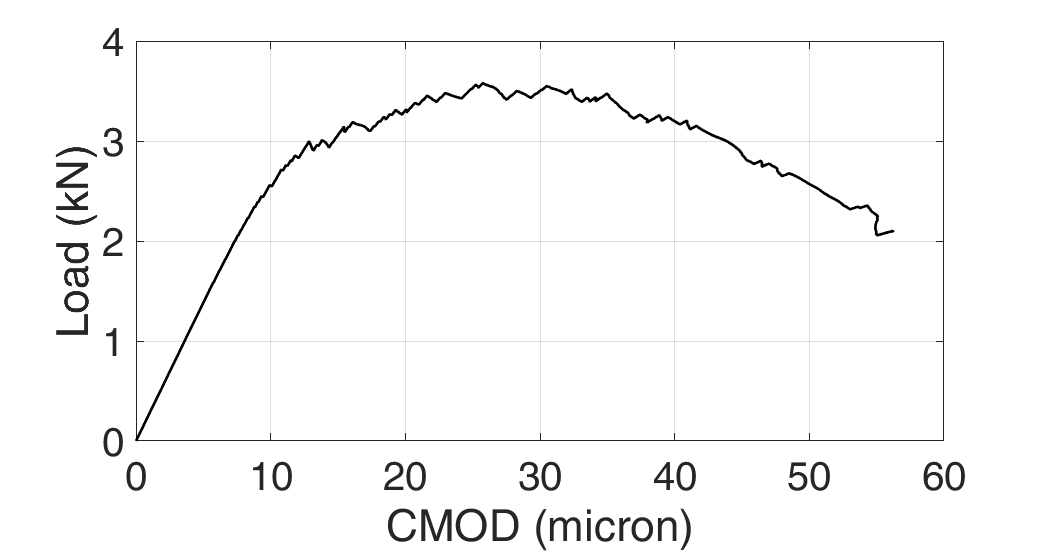
\includegraphics[width=0.75\textwidth]{figures/Amir_ME1_LEM_Displacement_Crystalline_Data.png}
\caption{The load vs. CMOD from the lattice simulation}
\label{fig:Amir_ME1_LEM_Displacement_Crystalline_Data}
\end{figure}

\subsubsection*{UFZ (FEM-VPF)}
The source code can be found in OpenGeoSys project on github and  the input files for the three point bending test performed on the Rockville Granite samples have been uploaded.
The files include the unstructured finite element mesh files in \texttt{vtu} format and an OGS input file in \texttt{xml} format.
As homogeneous properties such as Young's modulus are assigned int the computational domain, the spatially constant material properties are specified in the OGS input file rather than in the mesh file.
The load and crack mouth opening displacment computed from the simulations are shown in~\ref{fig:Keita_ME1_VPF_Rockville} as described in section \ref {sec:mex01}.

\begin{figure}[!ht]
\centering
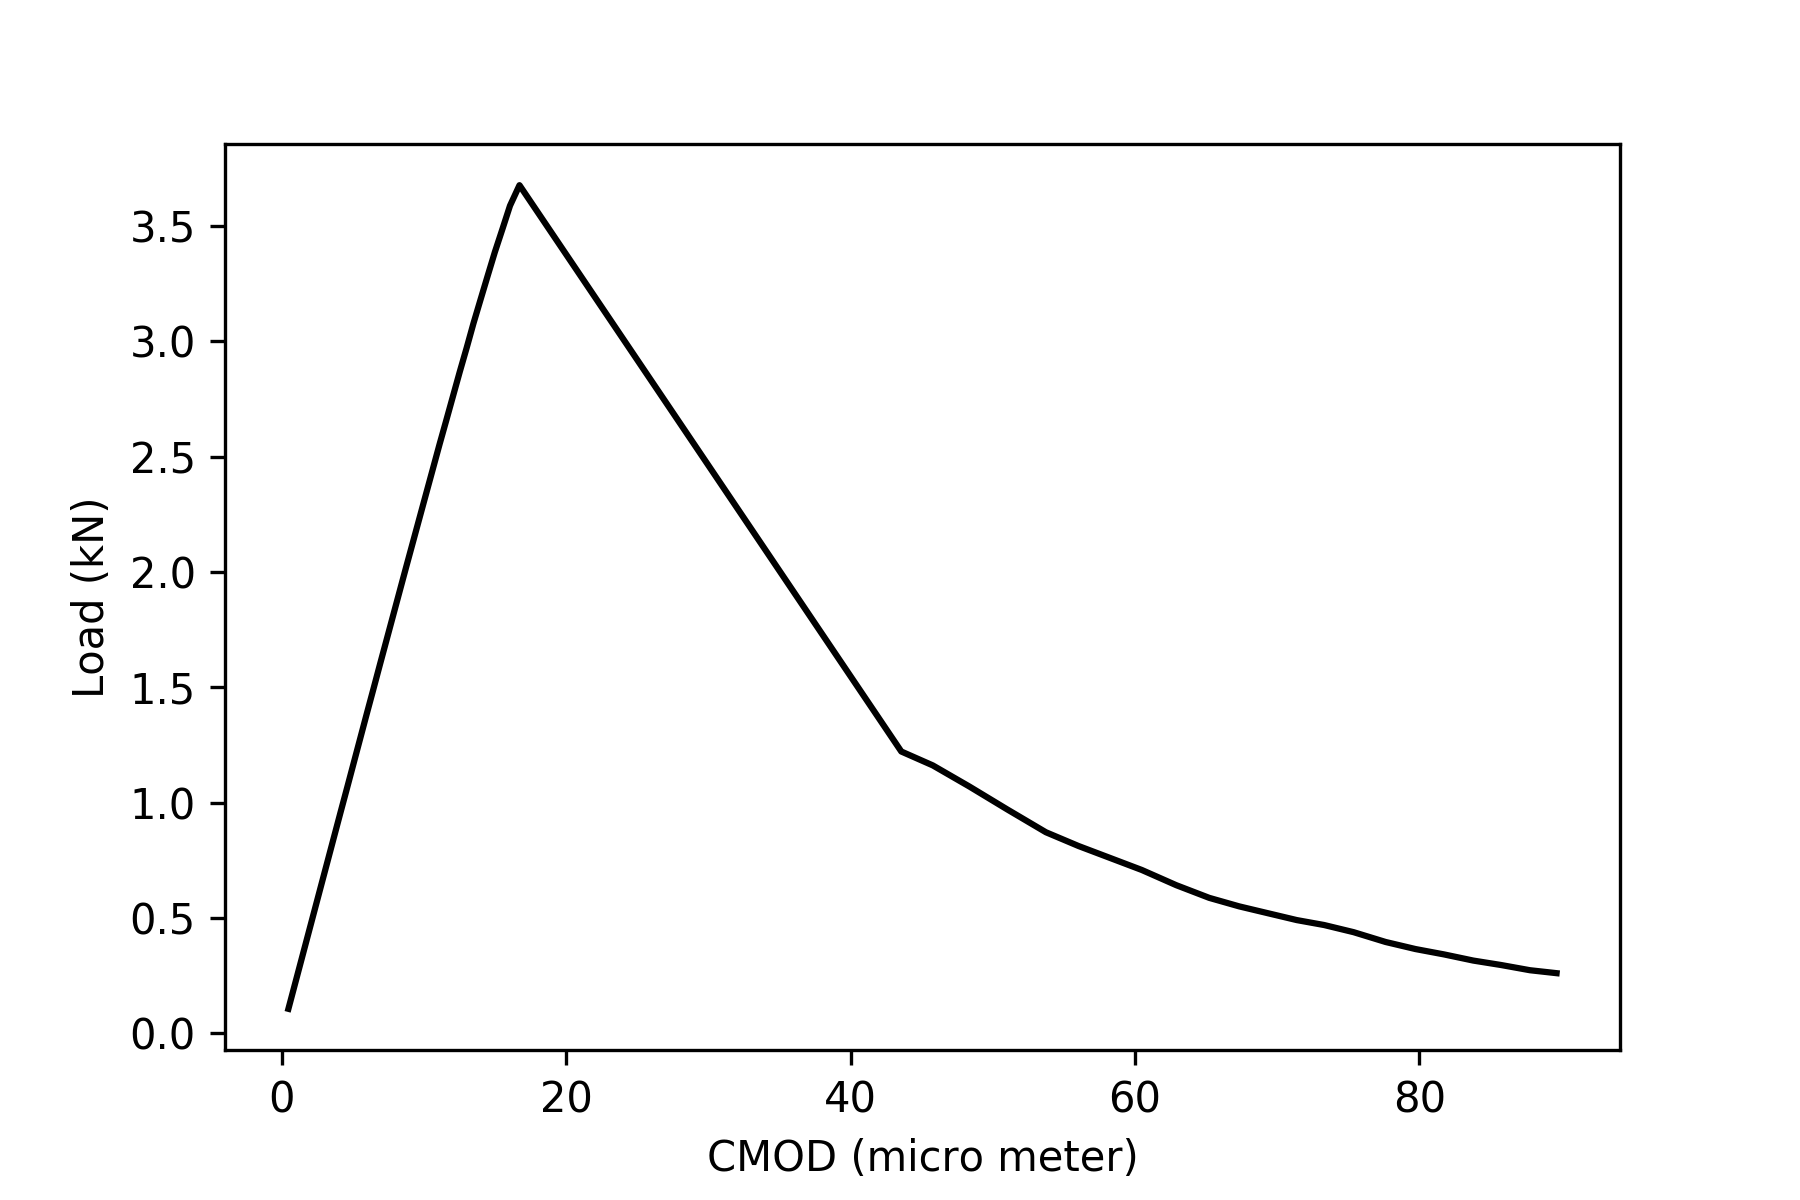
\includegraphics[width=0.75\textwidth]{figures/VPF_ME1_NF_CMOD.png}
\caption{The load vs. CMOD from the VPF simulation results}
\label{fig:Keita_ME1_VPF_Rockville}
\end{figure}

MEX 0-1a (UFZ) will be also provided as an OGS benchmark case at:\\
\small
\url{https://www.opengeosys.org/docs/benchmarks/phase-field/phasefield/}
\normalsize

\clearpage
%---------------------------------------------------------
\subsubsection*{Meta Data Overview (according to Dublin Core)}
%---------------------------------------------------------
\begin{table}[!ht]
\caption{MEX 0-1a (CAU)}
\label{tab:dms-mex0-1a-cau}
\small
\begin{tabular}{R{3.5cm}|L{7.5cm}}
\hline
%
Data label & GeomInt | CAU | Bending fracture test, Granite \\
URL (Numerics) &  \url{https://nextcloud.ifg.uni-kiel.de/index.php/s/pRmBPJ9gK5Se6ci} \\
Subject  &  LEM simulation of bending fracture test (Granite)\\
Type of data  &  Executable MATLAB P-file, input parameters\\
Data quality  &  Quality assured data \\
Status of data  &  Unprocessed data\\
Data format  & txt, MATLAB executable P-file\\
Creators  &  Kiel University, Institute of Geomechanics and Geotechnics, Ludewig-Meyn-Stra\ss e 10, 24118, Kiel\\
Source/Origin & In-house code \\
Publisher  &  Kiel University, Institute of Geomechanics and Geotechnics, Ludewig-Meyn-Stra\ss e 10, 24118, Kiel \\
Rights holders &  Kiel University, Institute of Geomechanics and Geotechnics, Ludewig-Meyn-Stra\ss e 10, 24118, Kiel \\
Contributors &   Kiel University, Institute of Geomechanics and Geotechnics: Amir Shoarian Sattari, Frank Wuttke\\
Time/period of creation &  2018-2019\\
Language of the content &  English\\
Update policy &  Stored data is final\\
Access permissions & Full access\\
%
\hline
\end{tabular}
\end{table}
%---------------------------------------------------------

%---------------------------------------------------------
\begin{table}[!ht]
\caption{MEX 0-1a (UFZ)}
\label{tab:dms-mex0-1a-ufz}
\small
\begin{tabular}{R{3.5cm}|L{7.5cm}}
\hline
%
Data label & MEX 0-1a (UFZ) \\
URL & \url{http://www.ufz.de/record/dmp/archive/7706} \\ 
Subject  & OGS-VPF simulation of bending fracture test (crystalline rock) \\
Type of data  & Data set (structured data in a defined format) \\
Data quality  & Quality assured data by benchmarking \\
Status of data  & Processed data \\
Data format  & OGS files \\
Creators  & Yoshioka, Keita  \\
Source/Origin & Open source \\
Publisher  & Helmholtz Centre for Environmental Research UFZ \\
Rights holders & Helmholtz Centre for Environmental Research UFZ \\
Contributors & Yoshioka, Keita \\
Time/period of creation & 2019-2020 \\
Language of content & English \\
Update policy & To be merged to OGS benchmarks (see below) \\
Access permissions & Free access \\
%
\hline
\end{tabular}
\end{table}
%---------------------------------------------------------

%---------------------------------------------------------
\begin{table}[!ht]
\caption{MEX 0-1a (IfG)}
\label{tab:dms-mex0-1a-ifg}
\small
\begin{tabular}{R{3.5cm}|L{7.5cm}}
\hline
%
Data label & MEX 0-1a (IfG) \\
URL &  \\ 
Subject  & DEM simulation of bending fracture test (crystalline rock) \\
Type of data  & Data set (structured data in a defined format) \\
Data quality  & Quality assured data by benchmarking \\
Status of data  &  \\
Data format  &  \\
Creators  & Nest, Mathias  \\
Source/Origin & Commercial code \\
Publisher  & Institut f\"u Gebirgsmechanik IfG \\
Rights holders & Institut f\"u Gebirgsmechanik IfG \\
Contributors & Nest, Mathias \\
Time/period of creation & 2019-2020 \\
Language of content & English \\
Update policy &  \\
Access permissions & Limited access \\
%
\hline
\end{tabular}
\end{table}

%ToDos
%\todo[inline]{The branch is not merged with the master yet. Files have been provided to data management.}
%\todo[inline]{[IfG] Please complete Meta Data  description}